\section{Results}

\begin{frame}{Results}
    \begin{table}[htb!]
        \centering
        \setlength{\tabcolsep}{1.5em}
        \renewcommand{\arraystretch}{1.5}
        \resizebox{0.98\textwidth}{!}{
        \begin{tabular}{l|ccc}
                               & counting              & shape                 & LEP \\
        \hline                                                                 
        w/o LFU &&& \\
        \hline
        $\BWe$      & $(11.16 \pm 0.04 \pm 0.27) \%$ & $(10.83 \pm 0.01 \pm 0.10) \%$  & $(10.71 \pm 0.14 \pm 0.07)$ \% \\
        $\BWm$      & $(11.13 \pm 0.03 \pm 0.21) \%$ & $(10.94 \pm 0.01 \pm 0.08) \%$ & $(10.63 \pm 0.13 \pm 0.07)$ \% \\
        $\BWt$      & $(10.64 \pm 0.08 \pm 0.65) \%$ & $(10.77 \pm 0.05 \pm 0.21) \%$ & $(11.38 \pm 0.17 \pm 0.11)$ \% \\
        $\BWh$      & $(67.08 \pm 0.07 \pm 0.72) \%$ & $(67.46 \pm 0.04 \pm 0.28) \%$ & $(-- \pm --)$ \% \\
        \hline
        w/ LFU &&& \\
        \hline
        $\BWl$      & $(-- \pm --)\%$       & $(10.89 \pm 0.01 \pm 0.08)\%$  & $(10.86 \pm 0.06 \pm 0.09)\%$  \\
        $\BWh$      & $(-- \pm --)\%$       & $(67.32 \pm 0.02 \pm 0.23)\%$  & $(67.41 \pm 0.18 \pm 0.20)\%$  \\
        \end{tabular}
        }
    \end{table}


    \begin{table}[htb!]
        \centering
        \renewcommand{\arraystretch}{1.5}
        \resizebox{0.7\textwidth}{!}{
        \begin{tabular}{ccc}
            counting              & shape                 & LEP \\
          $\begin{bmatrix} 1 &+0.59 &-0.06 \\  +0.59 &1 &-0.27 \\ -0.06 &-0.27 &1 \end{bmatrix}$  
        & $\begin{bmatrix} 1 &+0.47 &+0.09 \\  +0.47 &1 &+0.14 \\ +0.09 &+0.14 &1 \end{bmatrix}$ 
        & $\begin{bmatrix} 1 &+0.17 &-0.20 \\  +0.17 &1 &-0.12 \\ -0.20 &-0.12 &1 \end{bmatrix}$ \\
        \end{tabular}}
    \end{table}
\end{frame}

\footnotetext[1]{\tiny first and second uncertainties are statistical and systematic.}

\begin{frame}{Results}
    \begin{center}
    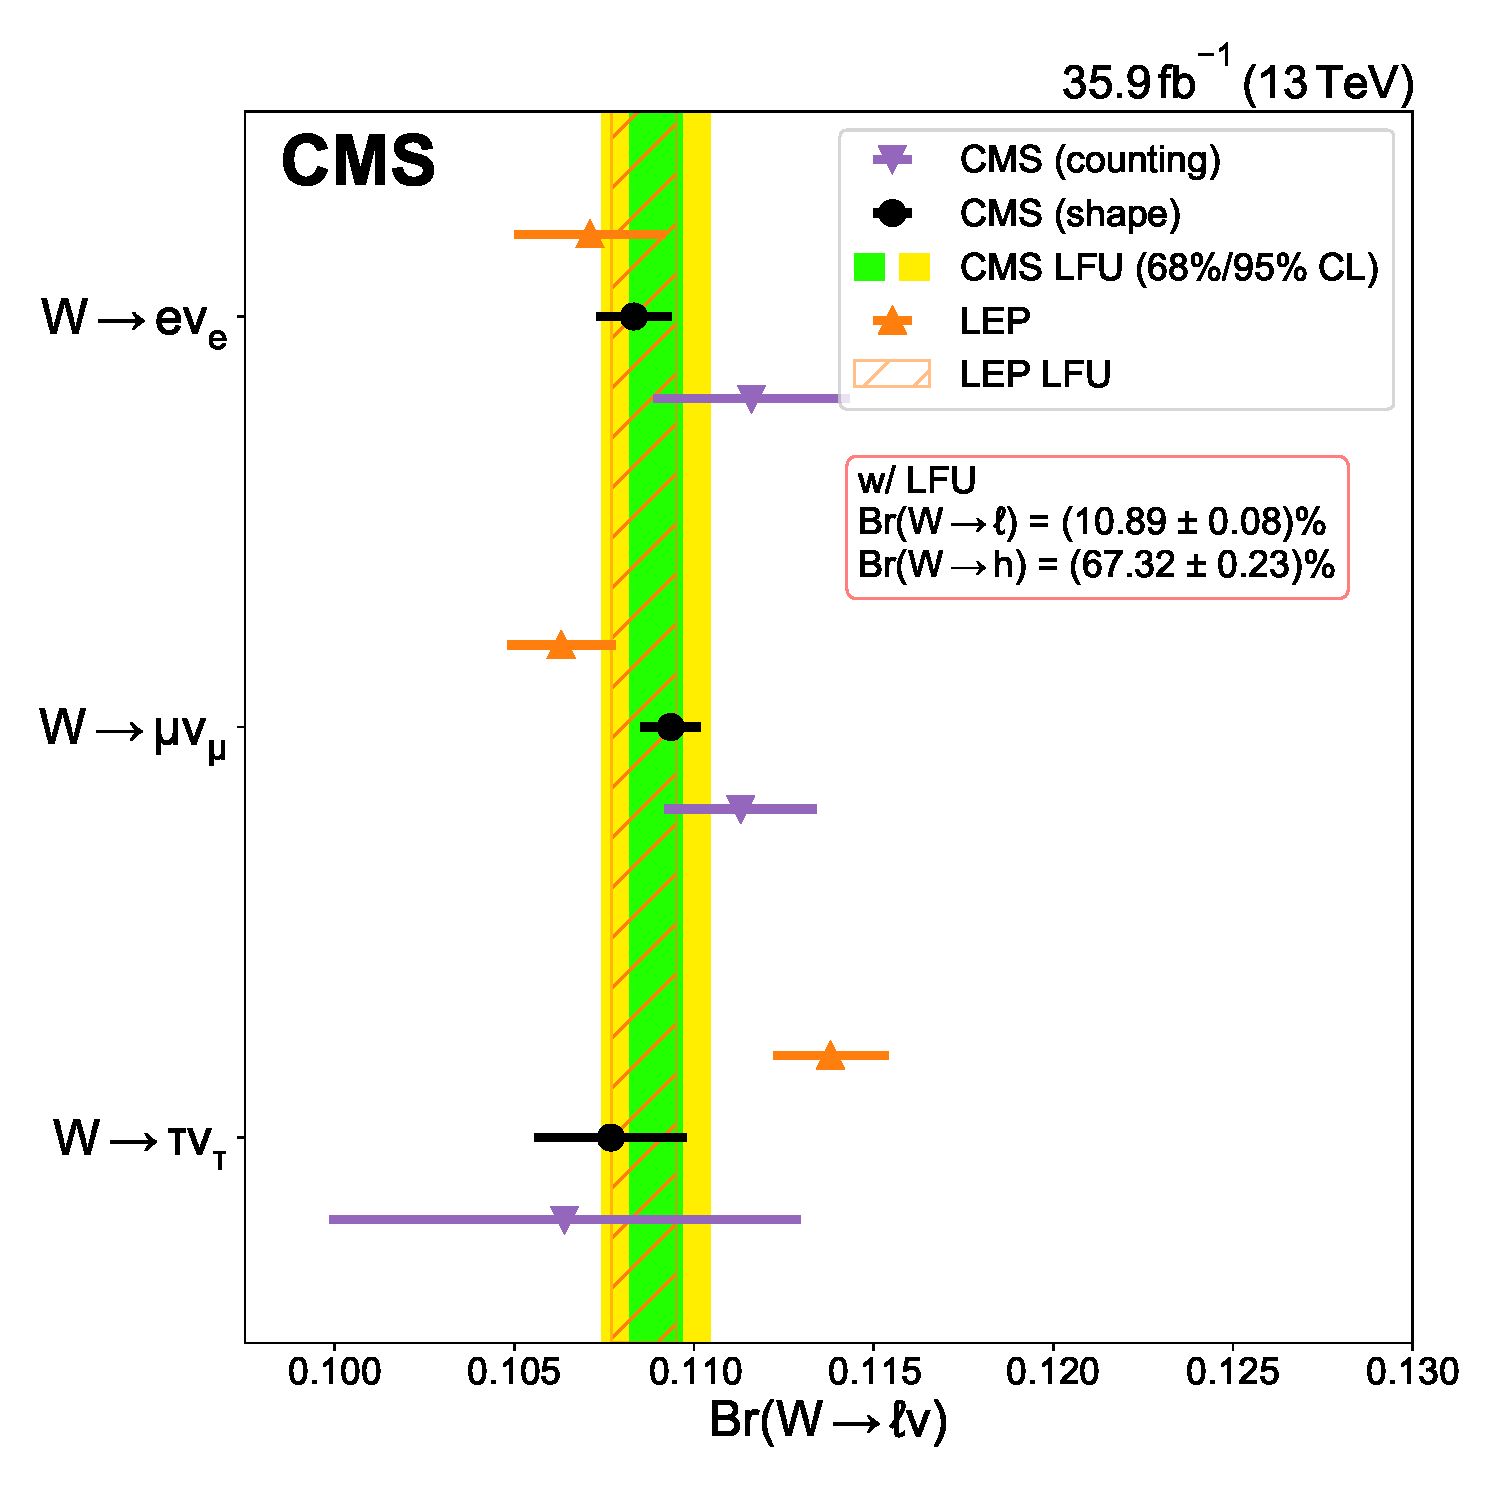
\includegraphics[width=0.5\textwidth]{chapters/Analysis/sectionResult/figures/unblinded_summary_plot.pdf}
    \end{center}
\end{frame}


\begin{frame}{Results}
    \begin{center}
    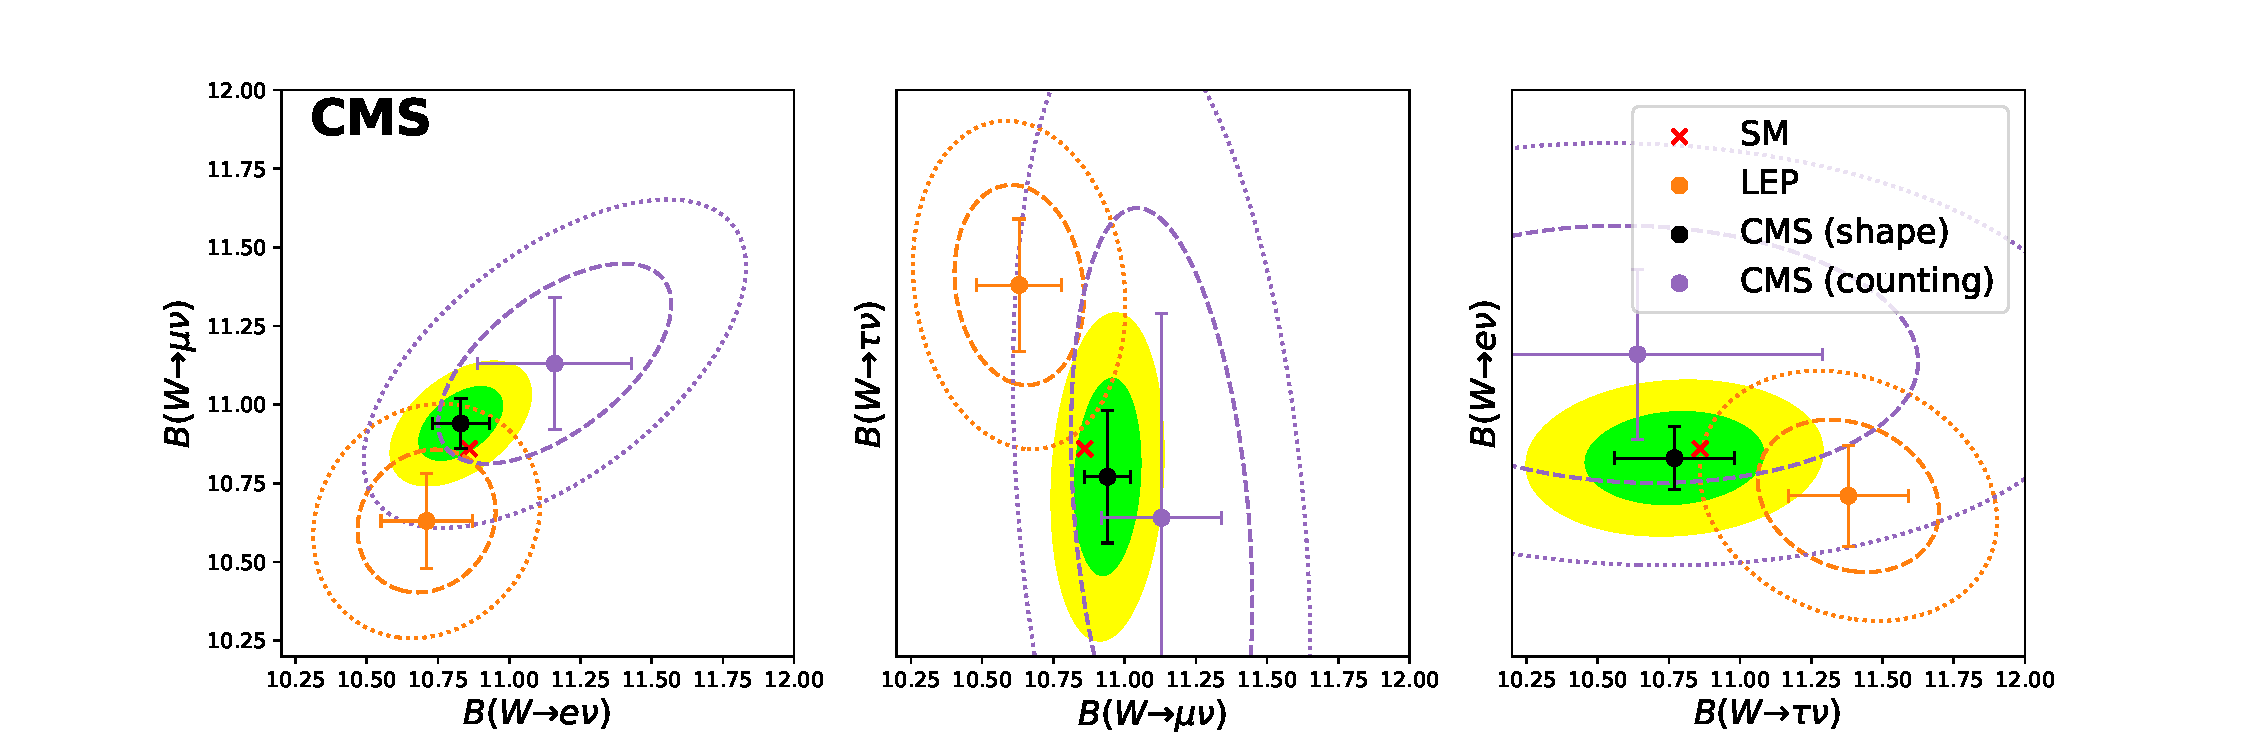
\includegraphics[width=0.99\textwidth]{chapters/Analysis/sectionResult/figures/result_contours_2d_br_dash.pdf}
    pair-wised \BWl on 2D plane. 68\%,95\% C.I. countours.
    \end{center}
\end{frame}

\begin{frame}{Results}
    \begin{center}
        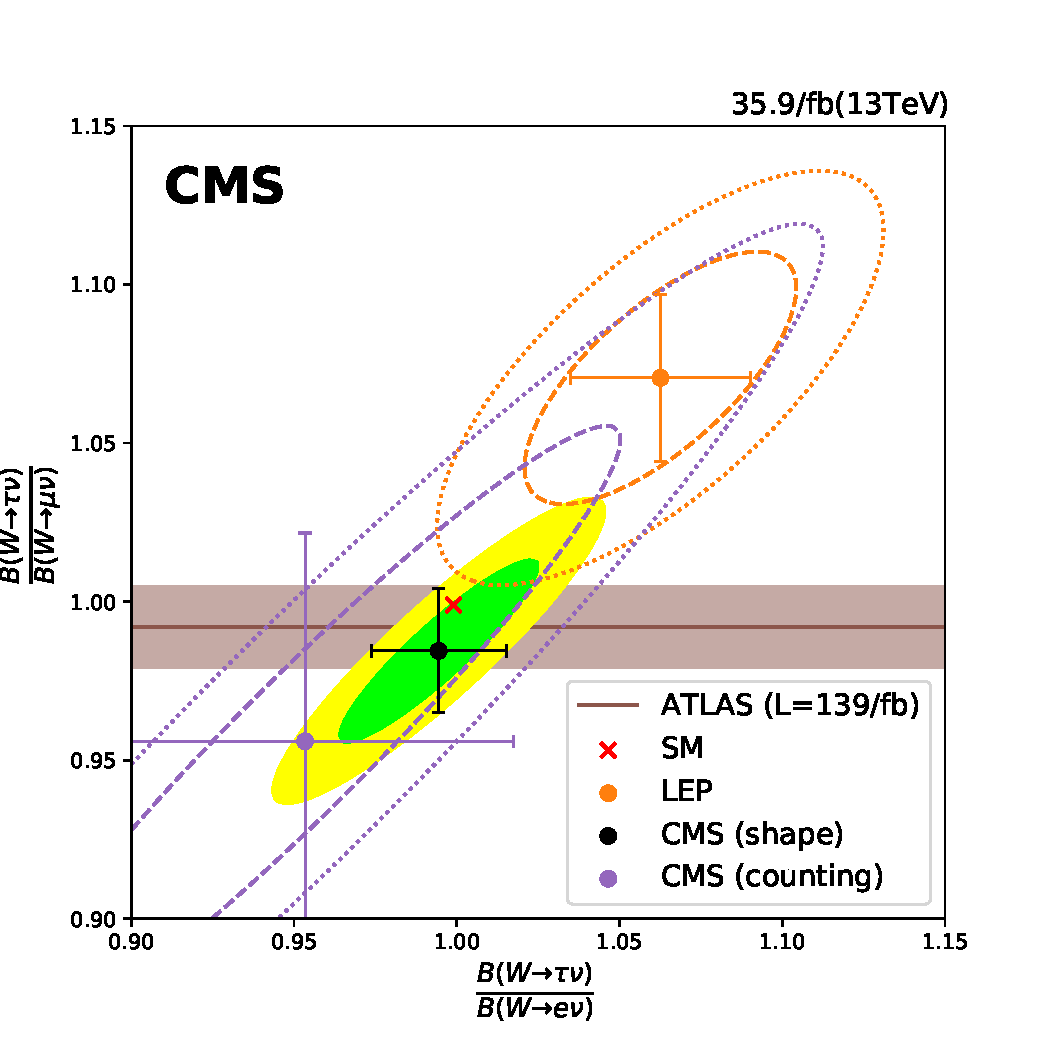
\includegraphics[width=0.6\textwidth]{chapters/Analysis/sectionResult/figures/result_contours_2d_ratio_symmetric.pdf}
    \end{center}
\end{frame}




\begin{frame}{\smaller More derived quantities from shape analysis}
    % \begin{equation}
    %     f(r_{\PGt/\Pe}, r_{\PGt/\PGm}) = \int_{-\infty}^{\infty}
    %     \left| \beta_{\PGt}\right|g(r_{\PGt/\Pe}\beta_{\PGt}, r_{\PGt/\PGm}\beta_{\PGt}, \beta_{\PGt})
    %     d\beta_{\PGt}
    % \end{equation}
    Assuming partial LFU between electron and muon, the shape analysis reperforms the fit with the same parameter for \BWe and \BWm.
    $$ 2 \BWt /(\BWe + \BWm) = 1.002(19) $$
    comparing with LEP's $1.066(25)$.
        
    
    % \begin{table}[htb!]
    %     \centering
    %     \setlength{\tabcolsep}{0.5em}
    %     \renewcommand{\arraystretch}{2}
    %     \resizebox{0.9\textwidth}{!}{
    %     \begin{tabular}{c|ccc}
    %                             & CMS               & LEP               & ATLAS              \\
    %     \hline                                                                 
    %     $\BWm / \BWe$           & $1.013 \pm 0.009$ & $0.993 \pm 0.019$ & --                 \\
    %     $\BWt / \BWe$           & $1.011 \pm 0.020$ & $1.063 \pm 0.027$ & --                 \\
    %     $\BWt / \BWm$           & $0.998 \pm 0.019$ & $1.070 \pm 0.026$ & $0.992 \pm 0.013$  \\
    %     $2 \BWt /(\BWe + \BWm)$ & $1.002 \pm 0.019$ & $1.066 \pm 0.025$ & --                 \\
    %     \end{tabular}}
    % \end{table}
\end{frame}







\begin{frame}{\smaller More derived quantities from shape analysis}
\smaller
\begin{center}
    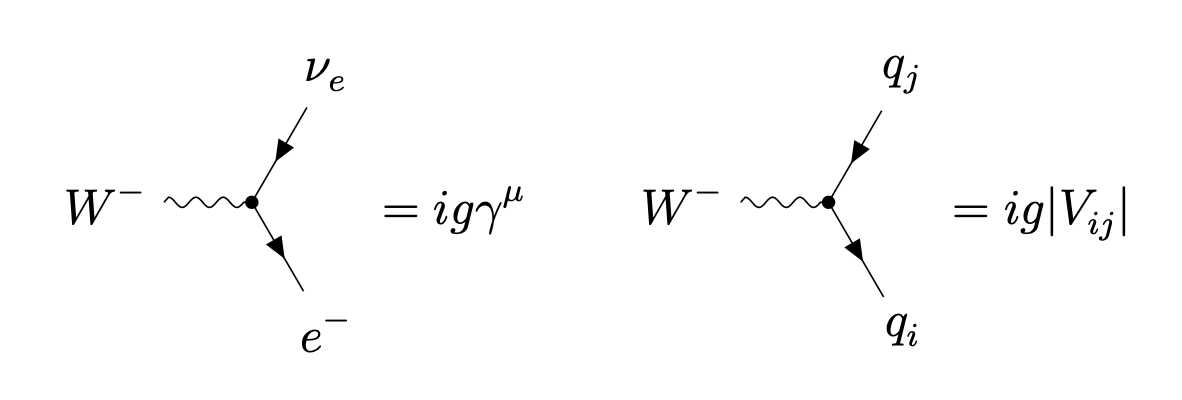
\includegraphics[width=0.5\textwidth]{slides/figures/ckm.png}
\end{center}

The CKM matrix is related to the ratio between the inclusive hadronic and inclusive leptonic branching fractions.

\begin{equation*}
\smaller \smaller \smaller 
    R^\PW_{\mathrm{h}/\ell} = \frac{\BWh }{\BWl} = \bigg( 1 + \frac{\alpS(m_\PW)}{\pi}\bigg) \sumCKM,
\end{equation*}


    \begin{table}[!h]
        \setlength{\tabcolsep}{0.5em}
        \renewcommand{\arraystretch}{1.2}
        \centering
        \resizebox{0.9\textwidth}{!}{
        \begin{tabular}{ccc|ccc}
            \hline
            Assumption &  &  Quantity & CMS & LEP & CMS+LEP\\
            \hline
                                                                &                   & $R^\PW_{\mathrm{h}/\ell}$ & $2.060\pm0.021$ & $2.068\pm0.025$ & $2.063\pm0.016$ \\ \hline
            CKM Unitarity: $\sumCKM = 2$                        & $\Longrightarrow$ & $\alpS(m_\PW)$            & $0.094\pm0.033$ & $0.108\pm0.040$ & $0.099\pm0.026$ \\ \hline
            PDG $\alpS(m_\PW) = 1.1200\pm0.010$  & $\Longrightarrow$ & \sumCKM                   & $1.985\pm0.021$ & $1.997\pm0.025$ & $1.992\pm0.016$ \\ \hline
            $\begin{matrix} 
                \text{PDG: } \alpS(m_\PW) = 1.1200\pm0.010 \\ 
                \text{PDG: } \sum_{\substack{ud,us,ub\\cd,cb}} |V_{ij}|^2 =1.0490(18) 
            \end{matrix} $ 
                                                                & $\Longrightarrow$ & \absVcs                   & $0.969\pm0.011$ & $0.974\pm0.013$ & $0.971\pm0.008$ \\ \hline
        \end{tabular}
        }
    \end{table}
\end{frame}

  
\begin{frame}{\smaller More derived quantities from shape analysis}
\smaller
    \begin{center}
    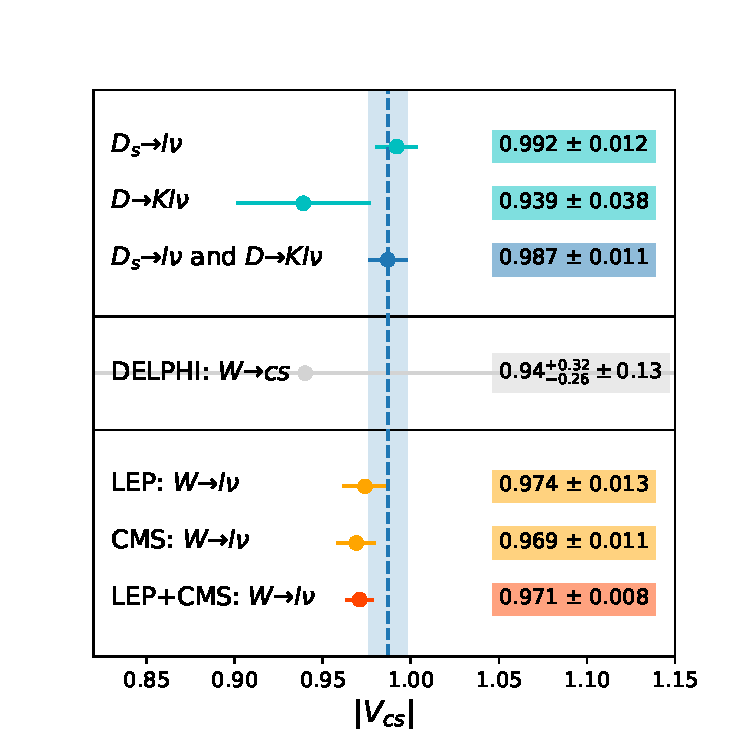
\includegraphics[width=0.5\textwidth]{chapters/Introduction/sectionRelatedWorks/figures/vcs.pdf}
    \end{center}
        
   
    Similar precision compare to the current \absVcs measurements. PDG average combines the measurements from
    \begin{itemize}
    \smaller
        \item $\PDs$ decay (Belle \cite{Zupanc:2013byn}, CLEO \cite{Alexander:2009ux,Onyisi:2009th,Naik:2009tk}, BaBar \cite{delAmoSanchez:2010jg} and BESIII \cite{Ablikim:2016duz, Ablikim:2018jun})
        \item $\PD$ decay (Belle \cite{Widhalm:2006wz}, CLEO \cite{Besson:2009uv}, BaBar \cite{Aubert:2007wg} and BESIII \cite{Ablikim:2015ixa, Ablikim:2018evp})
    \end{itemize}


\end{frame}


